\section{Приложение}
\label{sec:Appendix} \index{Appendix}

\textbf{
	\begin{large}
		Визуальные результаты работы моделей
	\end{large}
}

\begin{figure}[h]
\begin{subfigure}[b]{.5\textwidth}
	\centering
	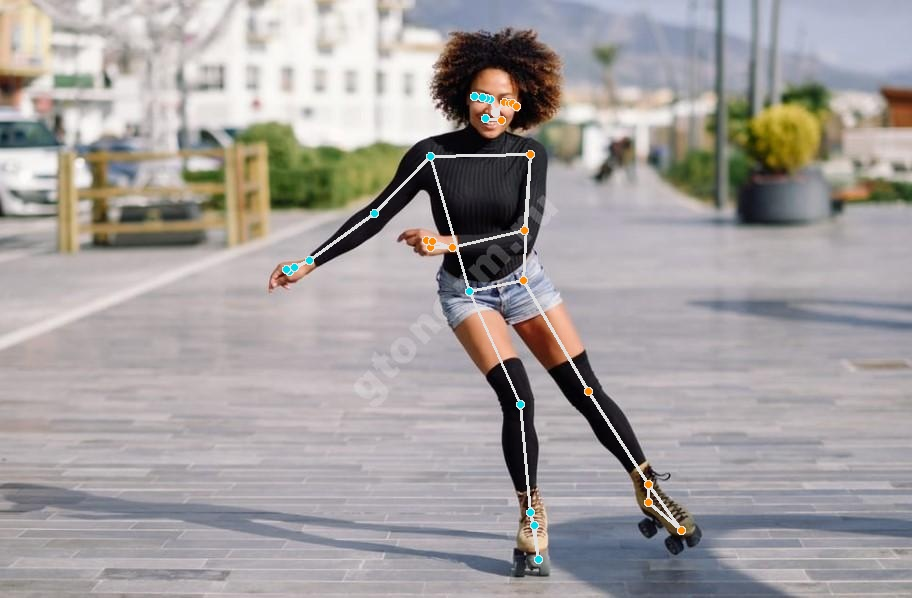
\includegraphics[width=\textwidth]{./images/MPPose/19}
	\caption{ }
\end{subfigure}
\begin{subfigure}[b]{.5\textwidth}
	\centering
   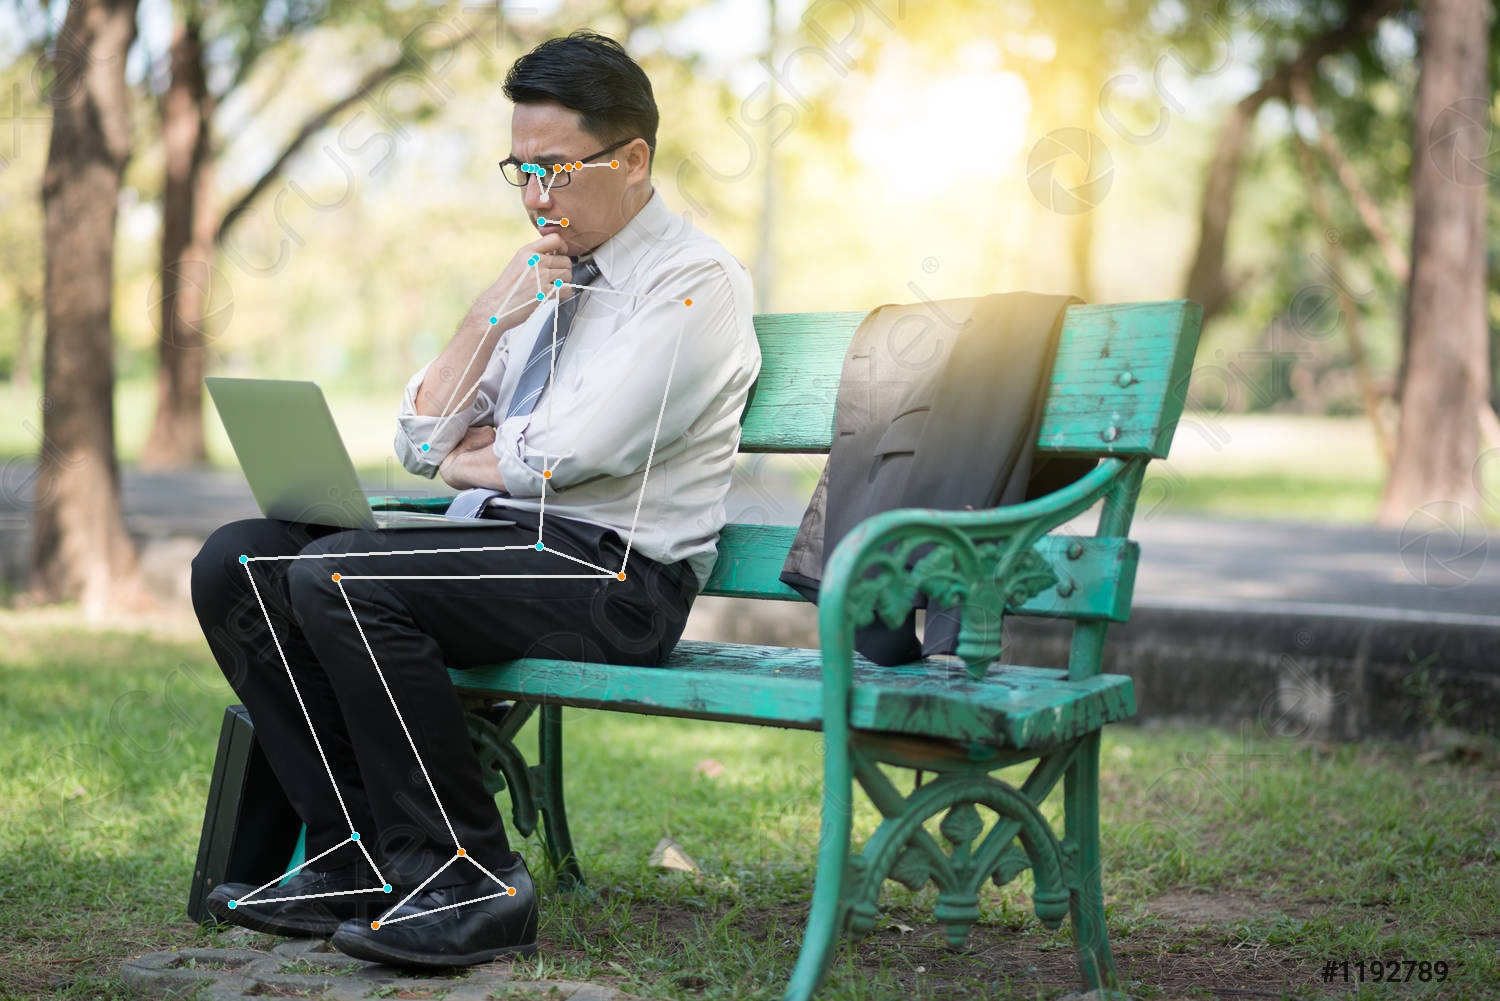
\includegraphics[width=\textwidth]{./images/MPPose/23}
   \caption{ }
\end{subfigure}
\begin{subfigure}[b]{.5\textwidth}
	\centering
   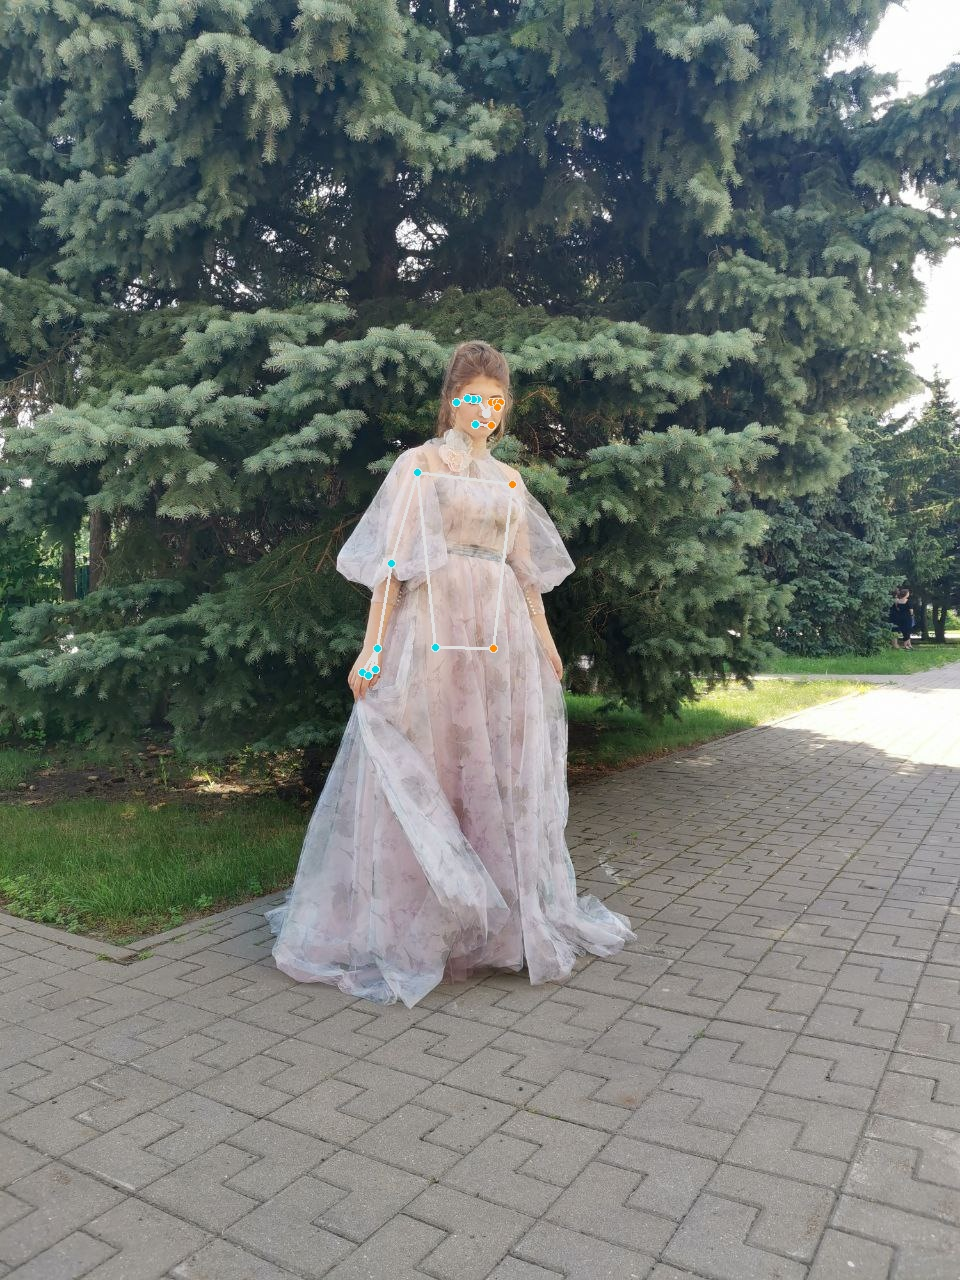
\includegraphics[height=\textwidth]{./images/MPPose/36}
   \caption{ }
\end{subfigure}
\begin{subfigure}[b]{.5\textwidth}
	\centering
   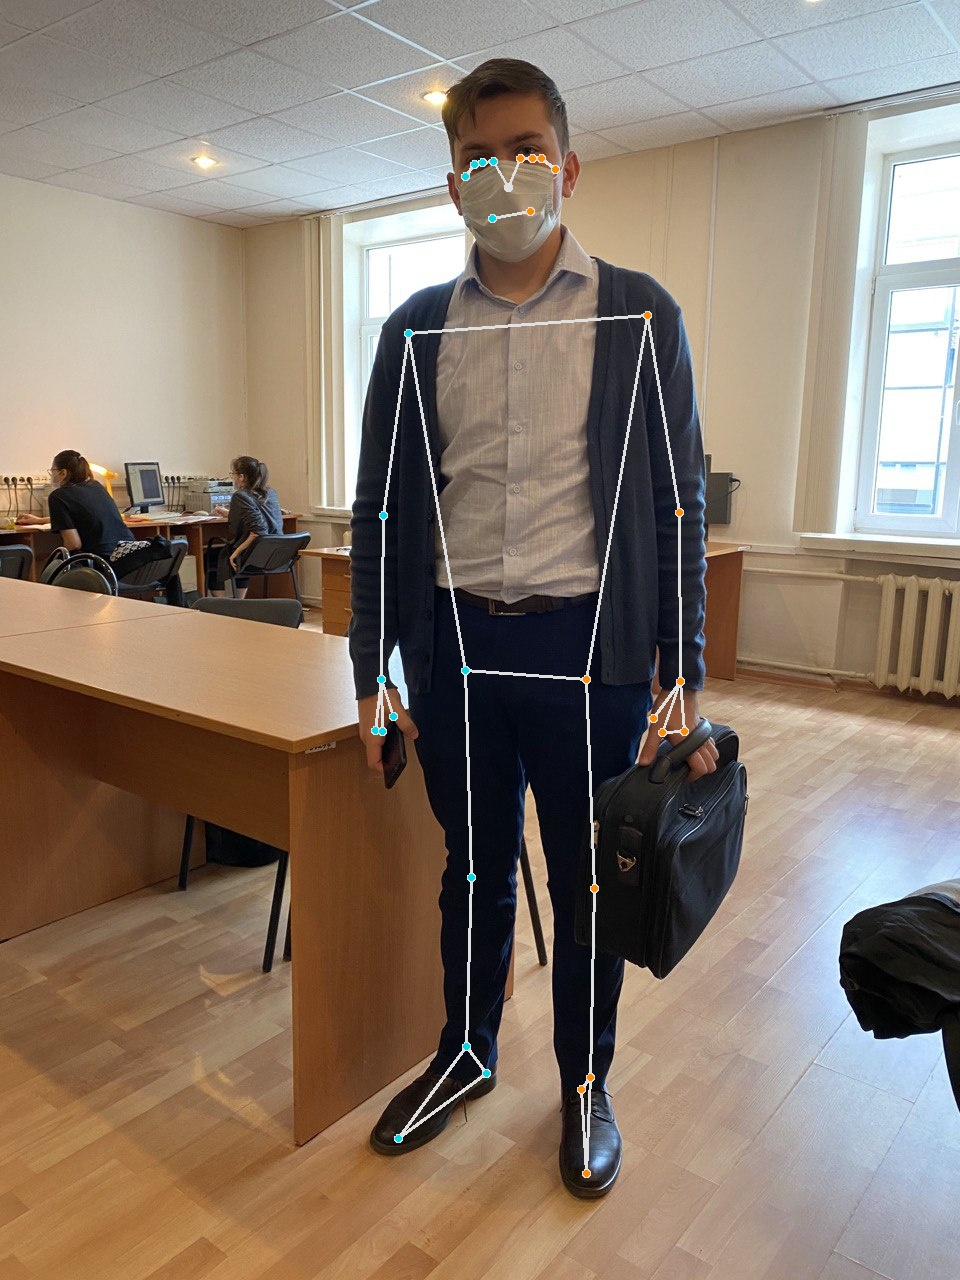
\includegraphics[height=\textwidth]{./images/MPPose/33}
   \caption{ }
\end{subfigure}
   \caption{Пример результатов работы модели BlazePose.}
   \label{fig:MP_result}
\end{figure}

\begin{figure}[h]
\begin{subfigure}[b]{.5\textwidth}
	\centering
	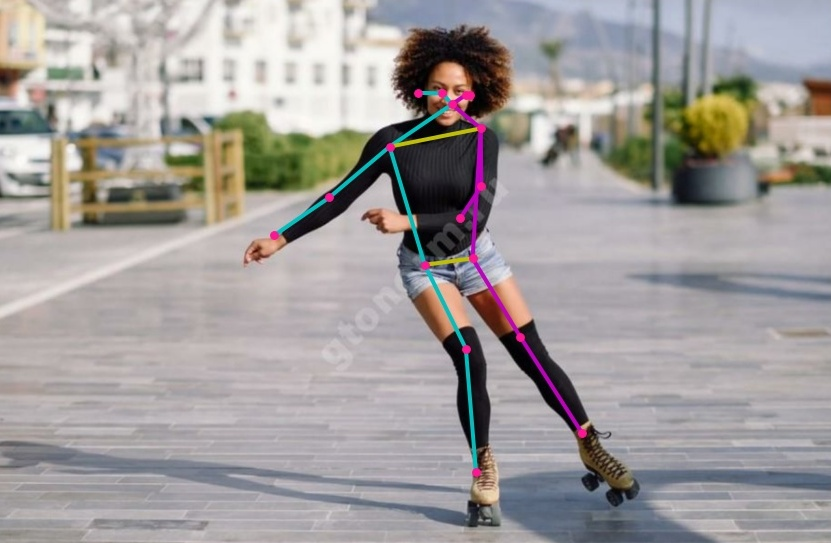
\includegraphics[width=\textwidth]{./images/MoveNet/19}
	\caption{ }
\end{subfigure}
\begin{subfigure}[b]{.5\textwidth}
	\centering
   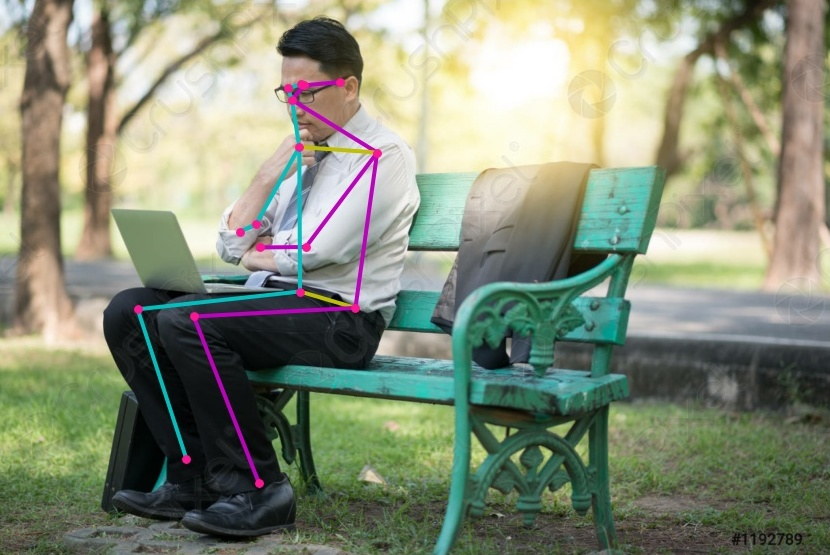
\includegraphics[width=\textwidth]{./images/MoveNet/23}
   \caption{ }
\end{subfigure}
\begin{subfigure}[b]{.5\textwidth}
	\centering
   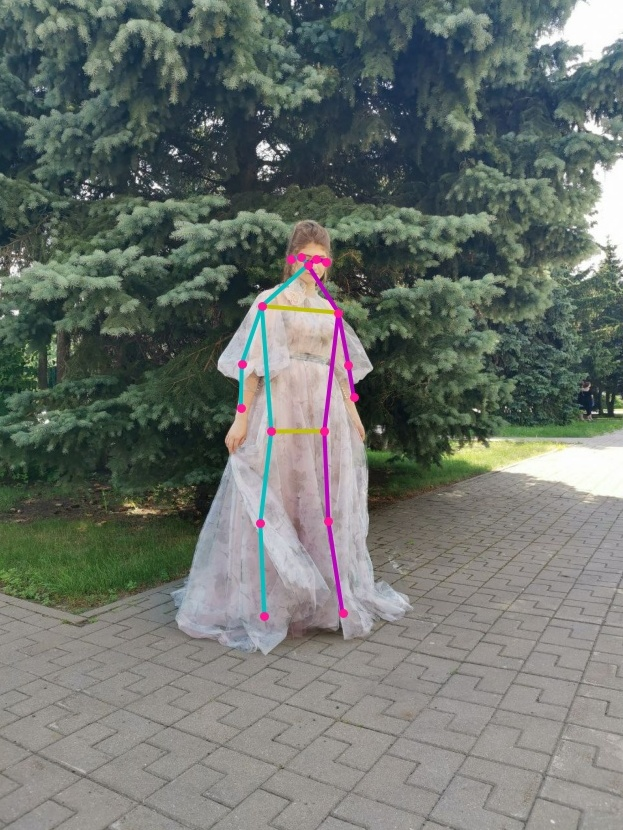
\includegraphics[height=\textwidth]{./images/MoveNet/36}
   \caption{ }
\end{subfigure}
\begin{subfigure}[b]{.5\textwidth}
	\centering
   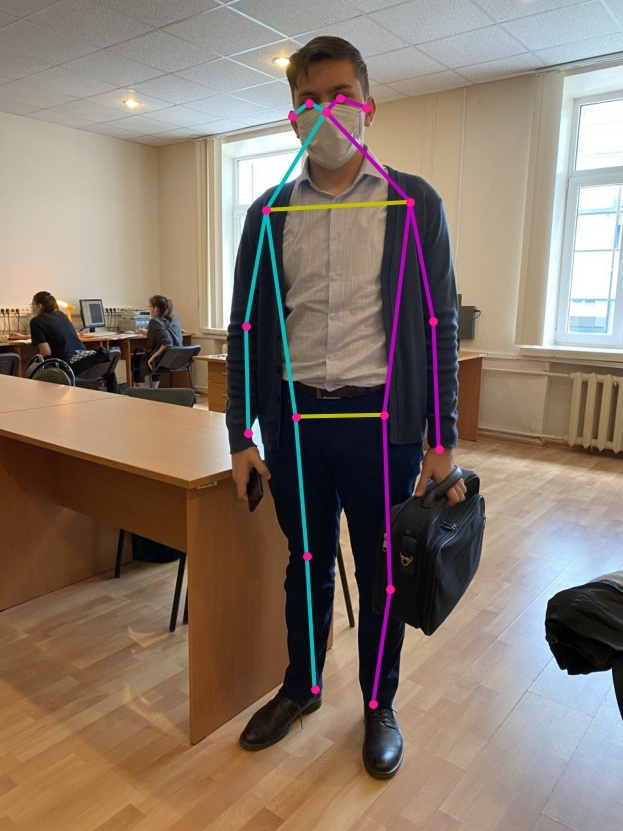
\includegraphics[height=\textwidth]{./images/MoveNet/33}
   \caption{ }
\end{subfigure}
   \caption{Пример результатов работы модели MoveNet.SinglePose.}
   \label{fig:MN_result}
\end{figure}

\begin{figure}[h]
\begin{subfigure}[b]{.5\textwidth}
	\centering
	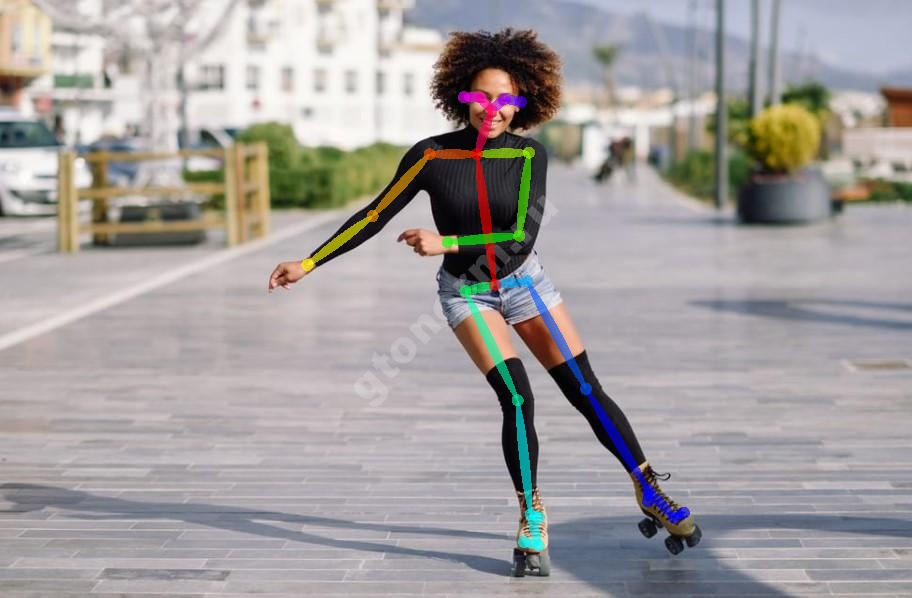
\includegraphics[width=\textwidth]{./images/OpenPose/19}
	\caption{ }
\end{subfigure}
\begin{subfigure}[b]{.5\textwidth}
	\centering
   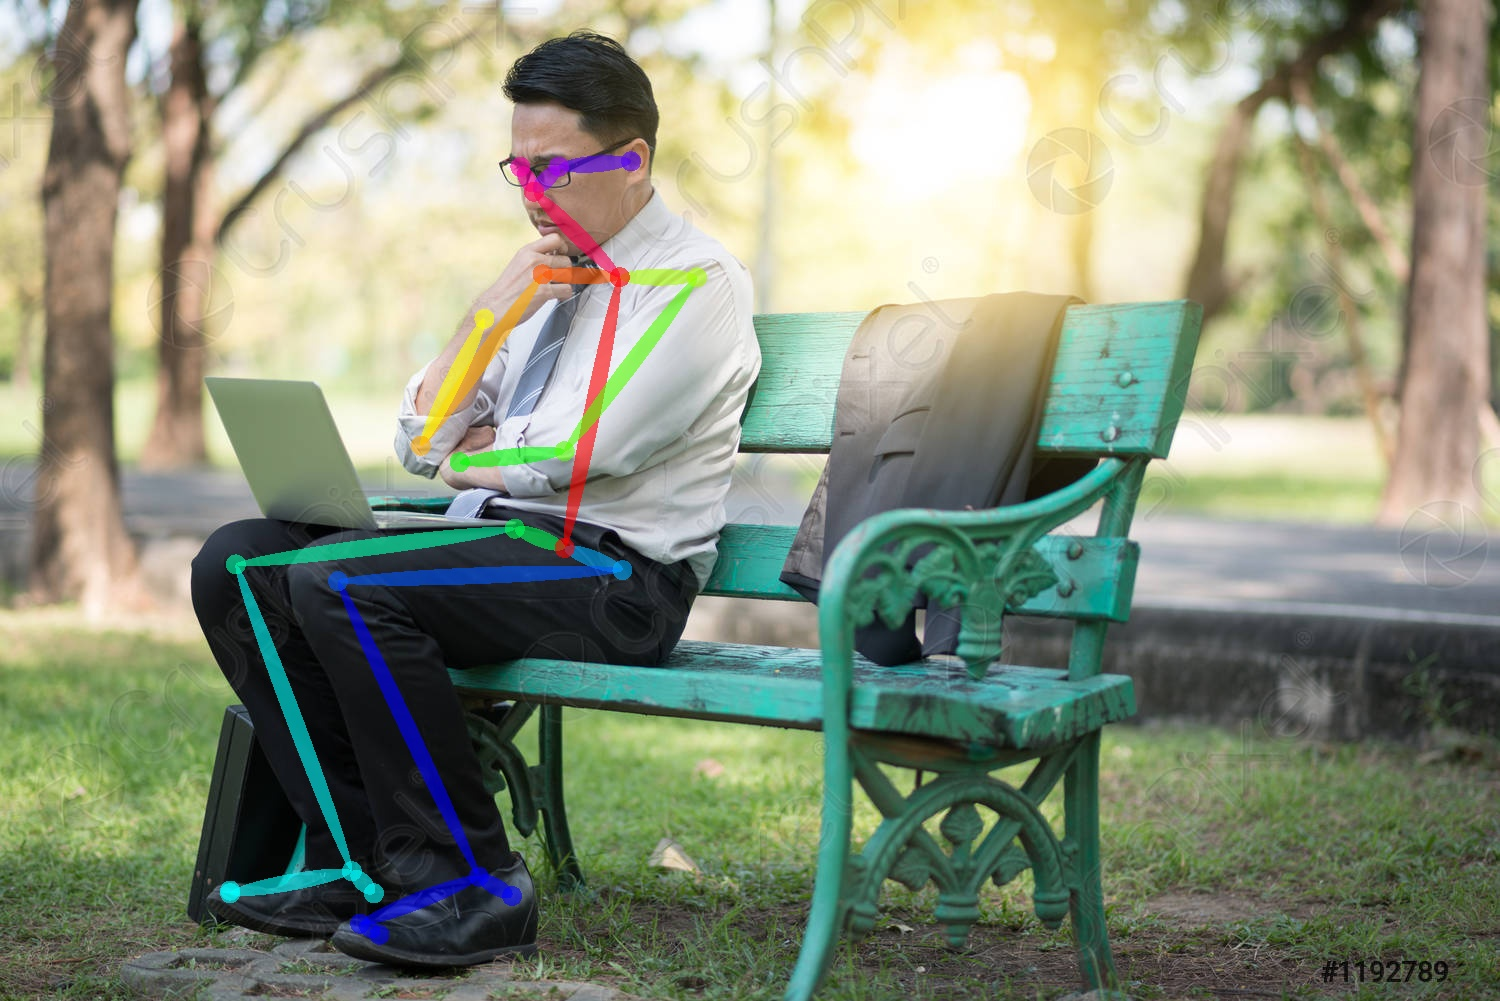
\includegraphics[width=\textwidth]{./images/OpenPose/23}
   \caption{ }
\end{subfigure}
\begin{subfigure}[b]{.5\textwidth}
	\centering
   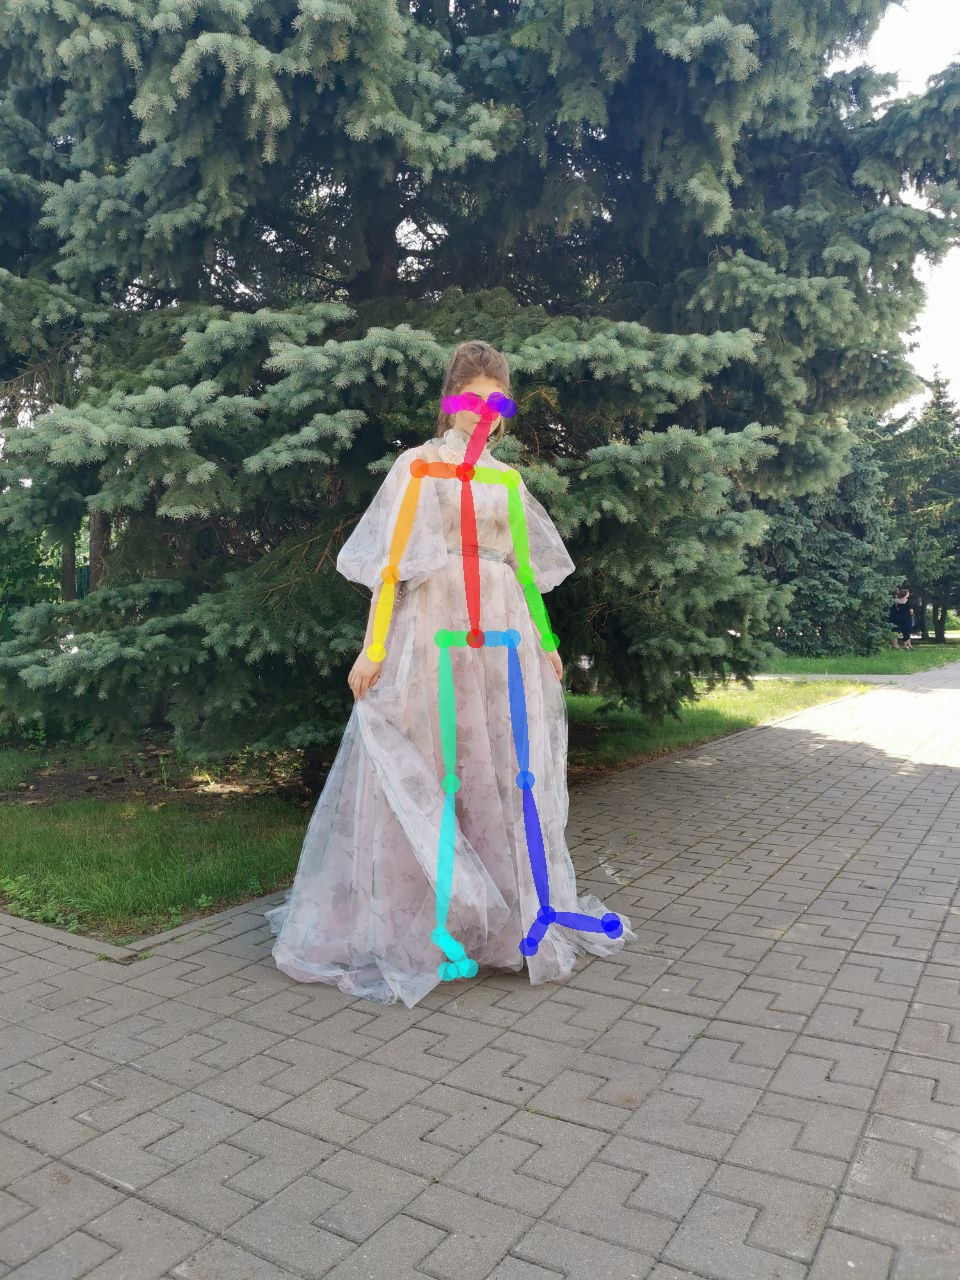
\includegraphics[height=\textwidth]{./images/OpenPose/36}
   \caption{ }
\end{subfigure}
\begin{subfigure}[b]{.5\textwidth}
	\centering
   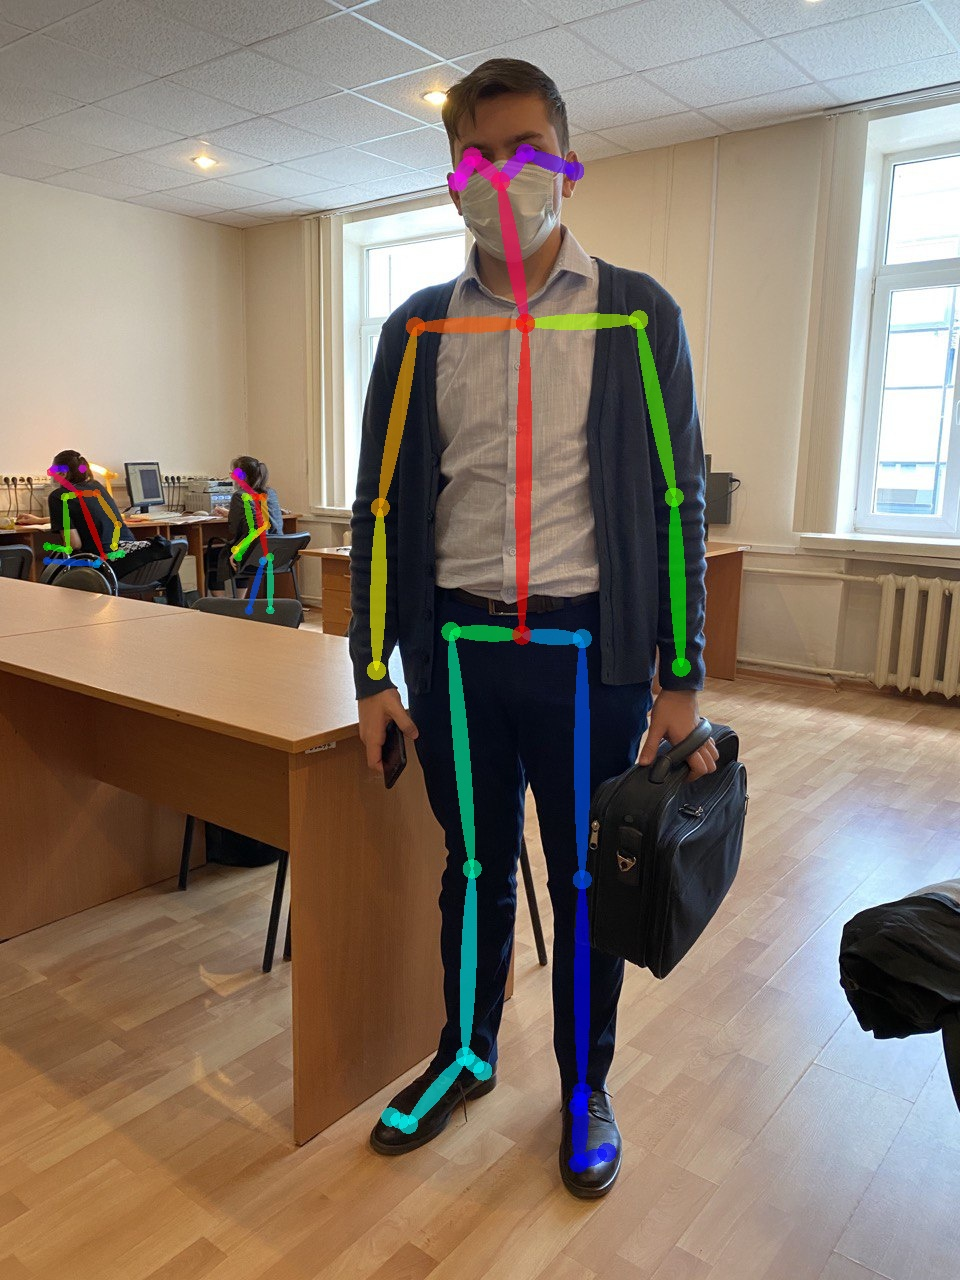
\includegraphics[height=\textwidth]{./images/OpenPose/33}
   \caption{ }
\end{subfigure}
   \caption{Пример результатов работы модели OpenPose.}
   \label{fig:OP_result}
\end{figure}

\begin{figure}[h]
\begin{subfigure}[b]{.5\textwidth}
	\centering
	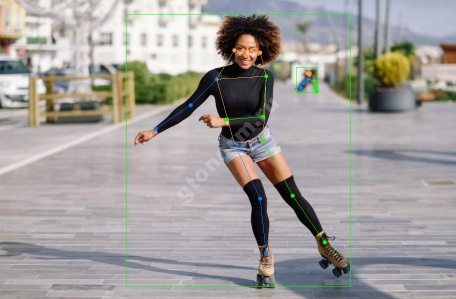
\includegraphics[width=\textwidth]{./images/MMPose/19}
	\caption{ }
\end{subfigure}
\begin{subfigure}[b]{.5\textwidth}
	\centering
   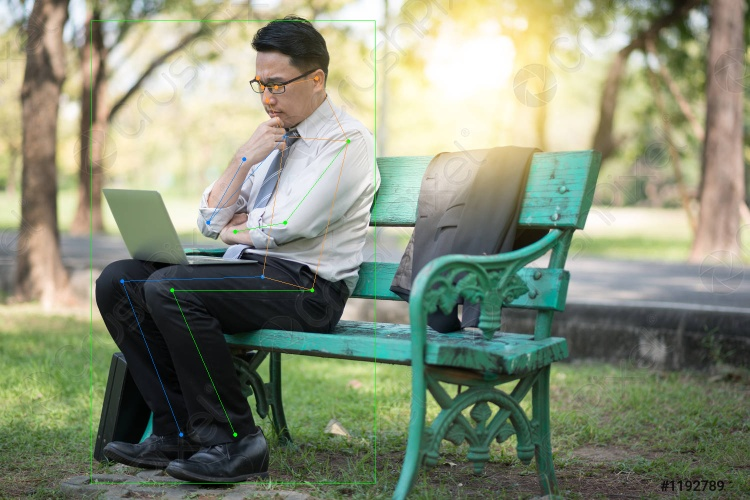
\includegraphics[width=\textwidth]{./images/MMPose/23}
   \caption{ }
\end{subfigure}
\begin{subfigure}[b]{.5\textwidth}
	\centering
   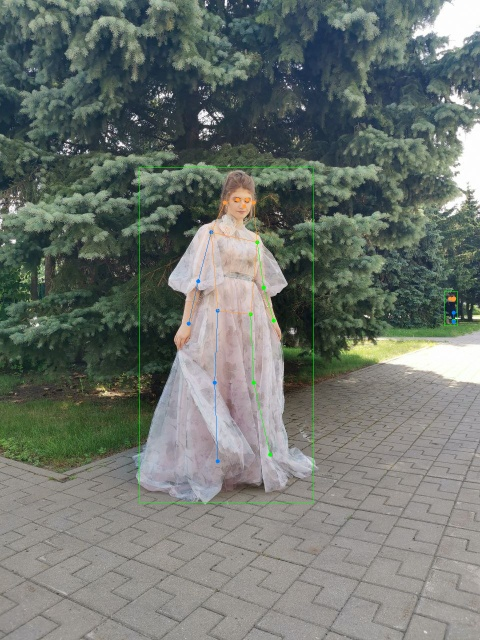
\includegraphics[height=\textwidth]{./images/MMPose/36}
   \caption{ }
\end{subfigure}
\begin{subfigure}[b]{.5\textwidth}
	\centering
   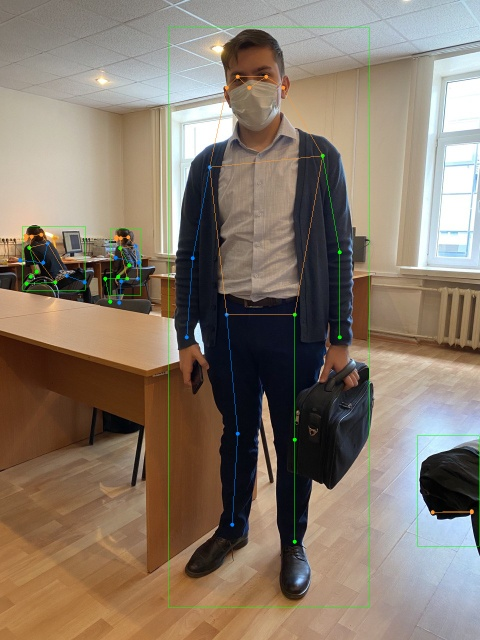
\includegraphics[height=\textwidth]{./images/MMPose/33}
   \caption{ }
\end{subfigure}
   \caption{Пример результатов работы модели MMPose.}
   \label{fig:MMP_result}
\end{figure}